\documentclass{../lab_class}

\usepackage{fancyhdr}
\pagestyle{fancy}
\rhead{П.\,Ю. Смирнов, 687 гр.}
\lhead{Лабораторная работа № 3.2.6, МФТИ, осень 2017}

\begin{document}

{\Large 3.2.6 -- Исследование гальванометра.}

\paragraph{Цель работы.}
Изучение работы высокочувствительного зеркального гальванометра магнитоэлектрической системы в режимах измерения постоянного тока и электрического заряда.

В работе используются: зеркальный гальванометр с осветителем и шкалой, источник постоянного напряжения, делитель напряжения, магазин сопротивления, конденсатор, вольметр, ключи, линейка.

\paragraph{Теоретическая часть.}

\begin{wrapfigure}[12]{r}{4.5cm}
	\centering
	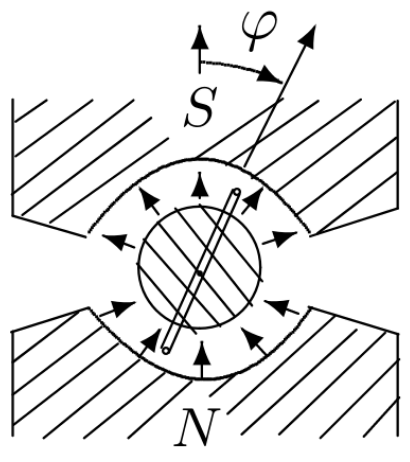
\includegraphics[width=3.2cm]{galvanometer.png}
	\caption{Рамка с током в магнитном поле}
	\label{fig:galvano}
\end{wrapfigure}

Баллистический гальванометр -- электроизмерительный прибор, принцип действия которого основан на измерении отклонения рамки с большим количеством витков при пропускании тока через них в радиальном поле внешнего постоянного магнита (см. рис. \ref{fig:galvano}). Если рассмотреть все моменты силы, действующие на обтекаемую током рамку, мы без особых трудностей (см. литературу) получим уравнение движения рамки:
\begin{equation}\label{eq:galvano_movement}
	\ddot{\varphi} + 2 \gamma \dot{\varphi} + \omega_0^2 \varphi = KI,
\end{equation}
где введены обозначения:
\begin{equation*}
	\frac{(BSN)^2}{JR} = 2 \gamma, \qquad \frac{D}{J} = \omega_0^2, \qquad \frac{BSN}{J} = K.
\end{equation*}
Это совершенно обычное дифференциальное уравнение движения <<богатой>> (на трение, внешнее воздействие, упругость и проч.) механической системы. Здесь $I$ -- пропускаемый через рамку ток, $R$ -- полное сопротивление цепи (включая сам прибор), остальное -- параметры самого гальвонометра, в том числе $B$ -- поле магнита, $S$ -- площадь витка, $N$ -- число витков, $J$ -- момент инерции рамки, $D$ -- модуль кручения нити. 

При измерениях баллистический гальванометр работает в двух режимах -- измерение постоянного тока и электрического заряда. В первом случае в уравнении \eqref{eq:galvano_movement} $\ddot{\varphi} = \dot{\varphi} = 0$, и угол поворота рамки определяется выражением
\begin{equation*}
	\varphi = \frac{BSN}{D} I = \frac{I}{C_I},
\end{equation*}
где введено обозначение $C_I$ -- \emph{динамическая постоянная} гальванометра. В случае же пропускания заряда делать это следует за промежуток времени меньший, чем период своодных колебаний рамки. Благо момент инерции рамки искусственно сделан весьма большим, тем самым увеличен период свободных колебаний и облегчен труд экспериментатора. 

Найдем скорость, приобретаемую рамкой в результате толчка, сообщаемым пропусканием заряда, проинтегрировав уравнение \eqref{eq:galvano_movement}. При этом полагаем $\varphi \approx \const$, поскольку время течения тока $\tau$ очень мало. Отсюда получаем
\begin{equation*}
	\dot{\varphi}(\tau) = Kq,
\end{equation*}
где $q$ -- измеряемый заряд. Наибольший угол отклонения, очевидно, также пропорционален заряду. Величину
\begin{equation*}
	C_Q = \frac{q}{\varphi_{max}}
\end{equation*}
называют \emph{баллистической постоянной} гальванометра.

Удобнее всего работать в \emph{критическом режиме} ($\gamma = \omega_0$), когда после начального импульса система достаточно быстро (экспоненциально) приближается к состоянию равновесия. Уравнение движения рамки при этом имеет вид $\varphi(t) = \dot{\varphi_0} t e^{-\gamma t}$. Сравнивая максимальное отклонение зайчика в режиме свободных колебаний (трение отсутствует) и в критическом режиме, получаем, что
\begin{equation*}
	\frac{C_{Q\text{крит}}}{C_{Q\text{своб}}} = e.
\end{equation*}

\paragraph{Экспериментальная установка.}

Для измерения отклонения рамки используется метод <<зайчика>>. Схемы используемых экспериментальных установок приведены на рисунках ниже и не представляют собой ничего сложного -- обычная электрическая цепь. При работе в баллистическом режиме источником измеряемых зарядов служит конденсатор, что является причиной обилия ключей на рис. \ref{fig:scheme_ball}.

\begin{figure}[H]
	\centering
	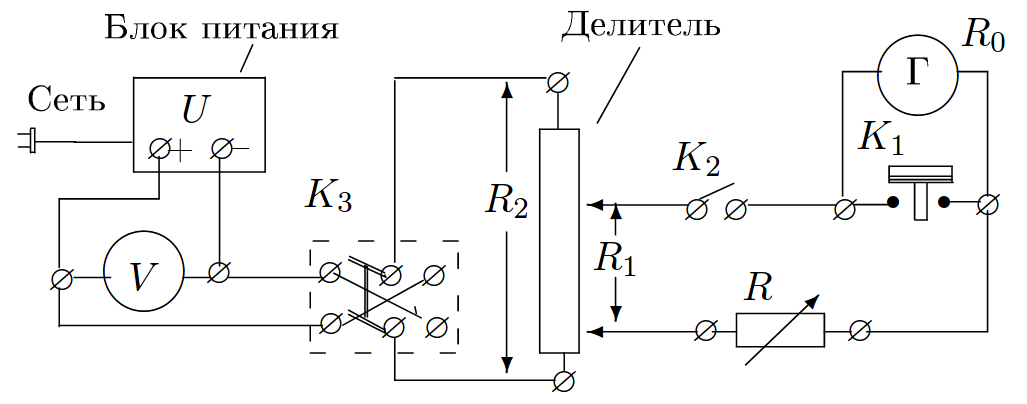
\includegraphics[width = 0.6 \textwidth]{scheme_st.png}
	\caption{Схема установки для исследования работы гальванометра в стационарном режиме}
	\label{fig:scheme_stat}
\end{figure}

\begin{figure}[H]
	\centering
	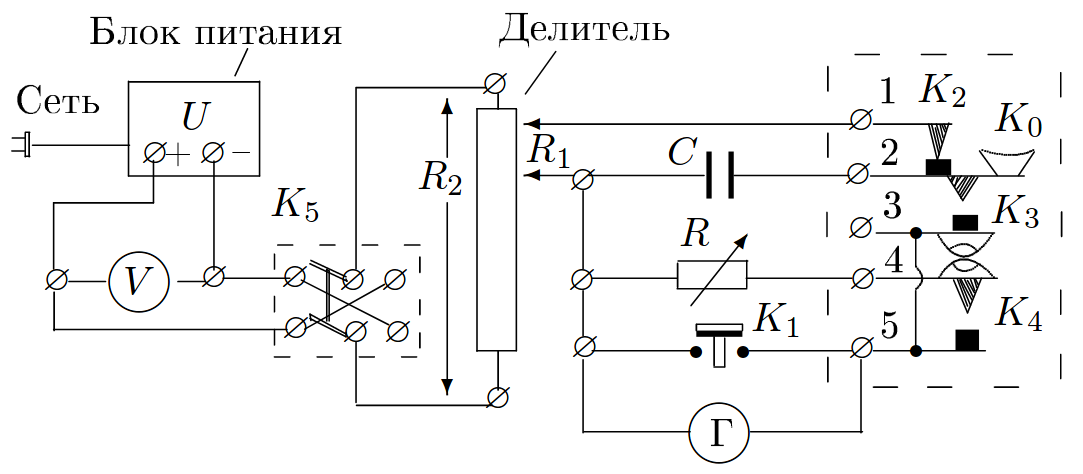
\includegraphics[width = 0.6 \textwidth]{scheme_ball.png}
	\caption{Схема установки для исследования работы гальванометра в баллистическом режиме}
	\label{fig:scheme_ball}
\end{figure}

\paragraph{Определение динамической постоянной.}
Работаем в стационарном режиме, используя установку, описанную на рис. \ref{fig:scheme_stat}. На блоке питания постоянное напряжение $U_0 \simeq 1.5 \ \V$. Сила тока через гальванометр определяется по формуле
\begin{equation*}
	I = U_0 \frac{R_1}{R_2} \frac{1}{R+R_0}, 
\end{equation*}
где $R_1/R_2 = 1/2000$ -- положение делителя, $R$ -- сопротивление магазина, $R_0 \simeq 610 \ \Ohm$ -- внутреннее сопротивление гальванометра. 

Отклонение светового пятна на шкале связано с поворотом рамки выражением
\begin{equation*}
	x = a \tan(2\varphi) \simeq 2 a \varphi,
\end{equation*}
где мы учли малость углов; $a \simeq 140 \ \cm$ -- расстояник от шкалы до зеркальца.

Построим зависимость $I = f(x)$, по наклону полученной прямой определим $C_I = 2aI/x$. 

\begin{table}[H]
	\centering
	\begin{tabular}{|c|c|c|c|c|c|c|c|c|c|c|}
																							  			  \hline
		$R$, \ \sk\Ohm 				& 3    & 3.5  & 4    & 4.5  & 5    & 6    & 7   & 10  & 15  & 20  \\ \hline
		$x$, \ \cm     				& 24.5 & 20.6 & 17.8 & 15.6 & 13.9 & 11.4 & 9.7 & 6.1 & 4.5 & 3.2  \\ \hline
		$I$, \ $10^{-8} \times \A$ & 21 & 18 & 16 & 15 & 13 & 11 & 10 & 7 & 5 & 4						  \\ \hline
	\end{tabular}
	\caption{Экспериментальные данные.}
\end{table}

\begin{figure}[H]
	\centering
	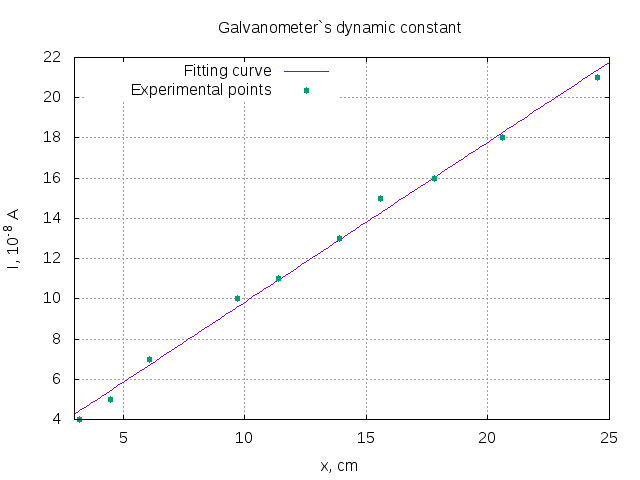
\includegraphics[width = 0.87 \textwidth]{dynamic_constant.png}
	\caption{К определению динамической постоянной гальванометра}
\end{figure}

Отсюда получаем динамическую постоянную:
\begin{gather*}
	C_I = (2.23 \pm 0.05) \times 10^{-11} \frac{\A}{\mm / \m}.
\end{gather*}

\paragraph{Определение критического сопротивления.}
Исследуем затухание в системе. При разомкнутой цепи имеем следующие последовательные положения зайчика при затухании:
\begin{table}[H]
	\centering
	\begin{tabular}{|c|c|c|c|c|}
		\hline
		$x$, \ \cm & 24.5 & 20.5 & 17.0 & 14.5 \\ \hline
	\end{tabular}
\end{table}
Отсюда 
\begin{gather*}
	\Theta_0 = \log{ \frac{x_n}{x_{n+1}} } = 0.17 \pm 0.01
\end{gather*}

Мы хотим найти критический режим, когда затухание происходит наиболее быстро, т.~е. $\Theta \to \infty$. Для систем с трением частота есть $\omega = \sqrt{\omega_0^2 - \gamma}$, потому
\begin{equation*}
	\Theta = \gamma T = \frac{2\pi\gamma}{\sqrt{\omega_0^2 - \gamma}} = \frac{2\pi R_3}{\sqrt{(R_0+R)^2 - R_3^2}},
\end{equation*} 
где введено обозначение
\begin{equation*}
	R_3 = \frac{(BSN)^2}{2\sqrt{JD}} = R_0 + R_{\text{крит}}.
\end{equation*}
Перепишем в виде
\begin{equation*}
	\frac{1}{\Theta^2} = \frac{(R_0+R)^2}{4\pi^2 R_3^2} - \frac{1}{4\pi^2};
\end{equation*}
критическое сопротивление можно определить по наклону графика $1/\Theta^2 = f[(R_0+R)^2]$:
\begin{equation*}
	R_{\text{крит}} = \frac{1}{2\pi} \sqrt{\frac{\Delta X}{\Delta Y}} - R_0.
\end{equation*}

\begin{table}[H]
	\centering
	\begin{tabular}{|c|c|c|c|c|}
		\hline
		$R$, \ \sk \Ohm & $x_0$ & $x_1$ & $x_2$ & $x_3$ \\ \hline
		21 & 16.9 & 14.5 & 12.4 & 10.5 \\ \hline
		28 & 12.7 & 10.6 & 9 & 7.6 \\ \hline
		35 & 10.2 & 8.5 & 7.6 & 6 \\ \hline
		42 & 8.5 & 7.1 & 6 & 5.1 \\ \hline
		56 & 6.4 & 5.5 & 4.6 & 3.9 \\ \hline
		70 & 5.2 & 4.4 & 3.8 & 3.3 \\ \hline
	\end{tabular}
	\caption{Затухание колебаний.}
\end{table}

\begin{figure}[H]
	\centering
	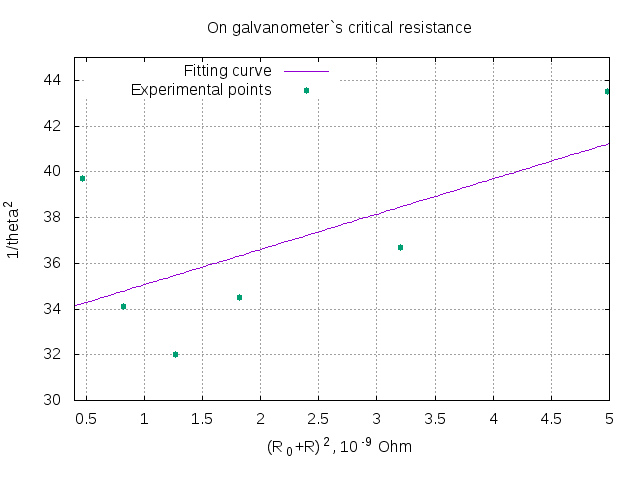
\includegraphics[width = 0.87 \textwidth]{critical_resistance.png}
	\caption{К определению критического сопротивления гальванометра}
\end{figure}

Отсюда получаем:
\begin{gather*}
	R_{\text{крит}} \simeq 2.6 \pm 0.2 \ \sk \Ohm
\end{gather*}
И вот уже постфактум оказывается, что работали мы совсем не в той области...

\pagebreak

\paragraph{Баллистический режим.}
В данном режиме мы пускаем заряд порциями, используя конденсатор $C = 2 \ \sn \F$. Работаем при положении делителя $R_1/R_2 = 1/20$. Ранее было установлено, что в критическом сопротивлении максимальное отклонение зайчика в $e$ раз меньше, чем при отсутствии затухания. Если $\gamma \ll \omega_0$, то
\begin{equation*}
	\varphi_1 = \varphi_0 e^{\Theta_0/4},
\end{equation*}
где $\varphi_1$ -- максимальное отклонение рамки при разомкнутой цепи, $\varphi_0$ -- максимальное отклонение без затухания. Используя данные соображения, по графику $l_{\text{max}} = f[(R_0+R)^{-1}]$ мы можем определить критическое сопротивление.
\begin{table}[H]
	\centering
	\begin{tabular}{|c|c|c|c|c|c|}
		\hline
		$R$, \ \sk \Ohm & 2 & 4 & 8 & 12 & 16 \\ \hline
		$l_{\text{max}}$, \ \cm & 5.2 & 9.5 & 12 & 14.5 & 14.5 \\ \hline
	\end{tabular}
\end{table}

\begin{figure}[H]
	\centering
	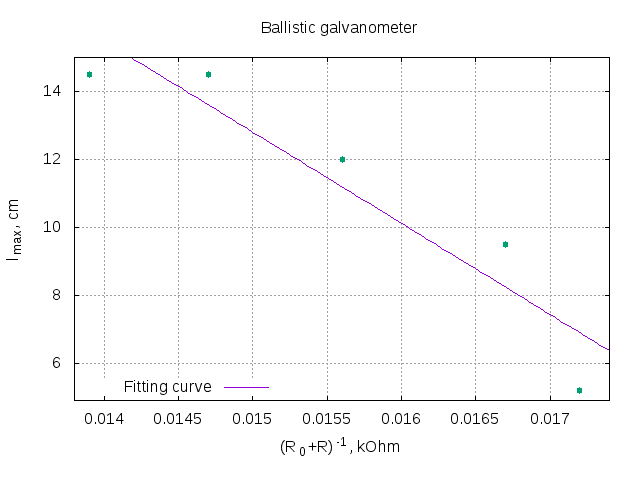
\includegraphics[width = 0.87 \textwidth]{ballistic.png}
	\caption{К определению критического сопротивления гальванометра в баллистическом режиме}
\end{figure}

\begin{gather*}
	R_{\text{крит}} \simeq 2.7 \pm 0.5 \ \sk \Ohm
\end{gather*}

Мы видим, что полученный результат согласуется с измерением в стационарном режиме, хотя имеет большую погрешность.

Определим баллистическую постоянную гальванометра (по-прежнему $a = 140 \ \cm$):
\begin{equation*}
	C_{Q\text{крит}} = \frac{q}{\varphi_{\text{max}}} = 2a \frac{R_1}{R_2} \frac{U_0 C}{l_{\text{max крит}}} \simeq (2.03 \pm 0.4) \times 10^{-9} \frac{\K}{\mm / \m}.
\end{equation*}

\paragraph{Выводы.}
Изучена работа гальванометра в стационарном и баллистическом режимах. Найдены экспериментально его параметры:
\begin{gather*}
	C_I = (2.23 \pm 0.05) \times 10^{-11} \frac{\A}{\mm / \m}, \\
	R_{\text{крит стац}} \simeq 2.6 \pm 0.2 \ \sk \Ohm, \\
	R_{\text{крит балл}} \simeq 2.7 \pm 0.5 \ \sk \Ohm, \\ 
	C_{Q\text{крит}} = (2.03 \pm 0.4) \times 10^{-9} \frac{\K}{\mm / \m}.
\end{gather*}

\end{document}